\documentclass[11pt, oneside]{article}
\usepackage[margin=0.75in]{geometry}
\geometry{letterpaper}
\usepackage{amssymb}
\usepackage[fleqn]{amsmath}
\usepackage[sharp]{easylist}
\usepackage{relsize}
\usepackage{graphicx}
\usepackage{enumitem}

\pagenumbering{gobble}              % No page numbering
\setlength{\parindent}{0em}         % No paragraph indenting
\setlength{\parskip}{0.5em}         % Paragraph spacing

\newcommand*{\begineasylist}{\begin{easylist}[itemize]\ListProperties(Style*=$\bullet$\quad, Style2*=\tiny$\blacksquare$\quad, Style3*=$\circ$\quad, Style4*=$\diamond$\quad, FinalSpace=1em, Space=-0.2em, Space*=-0.2em)}

\newcommand*{\begineasylistnumbered}{\begin{easylist}[enumerate]\ListProperties(Numbers=a, Space=0em, Space*=0em)}

\newcommand*{\un}[1]{\underline{\smash{#1}}}        % custom underline macro

\newenvironment{itemized}{\begin{itemize}[noitemsep, topsep=0pt, leftmargin=*]}{\end{itemize}}  % cusom itemize environment

\begin{document}

\section*{CS 349 Midterm Review}

\subsection*{Background \& History}
\begineasylist

# \textbf{User interface}: 
## The place where a person \un{expresses intention} to an artifact, and the artifact \un{presents feedback} to the person
## The way people (mental model) and technology (system model) interact

## Represented as MVC: \\
% \begin{figure}[h]
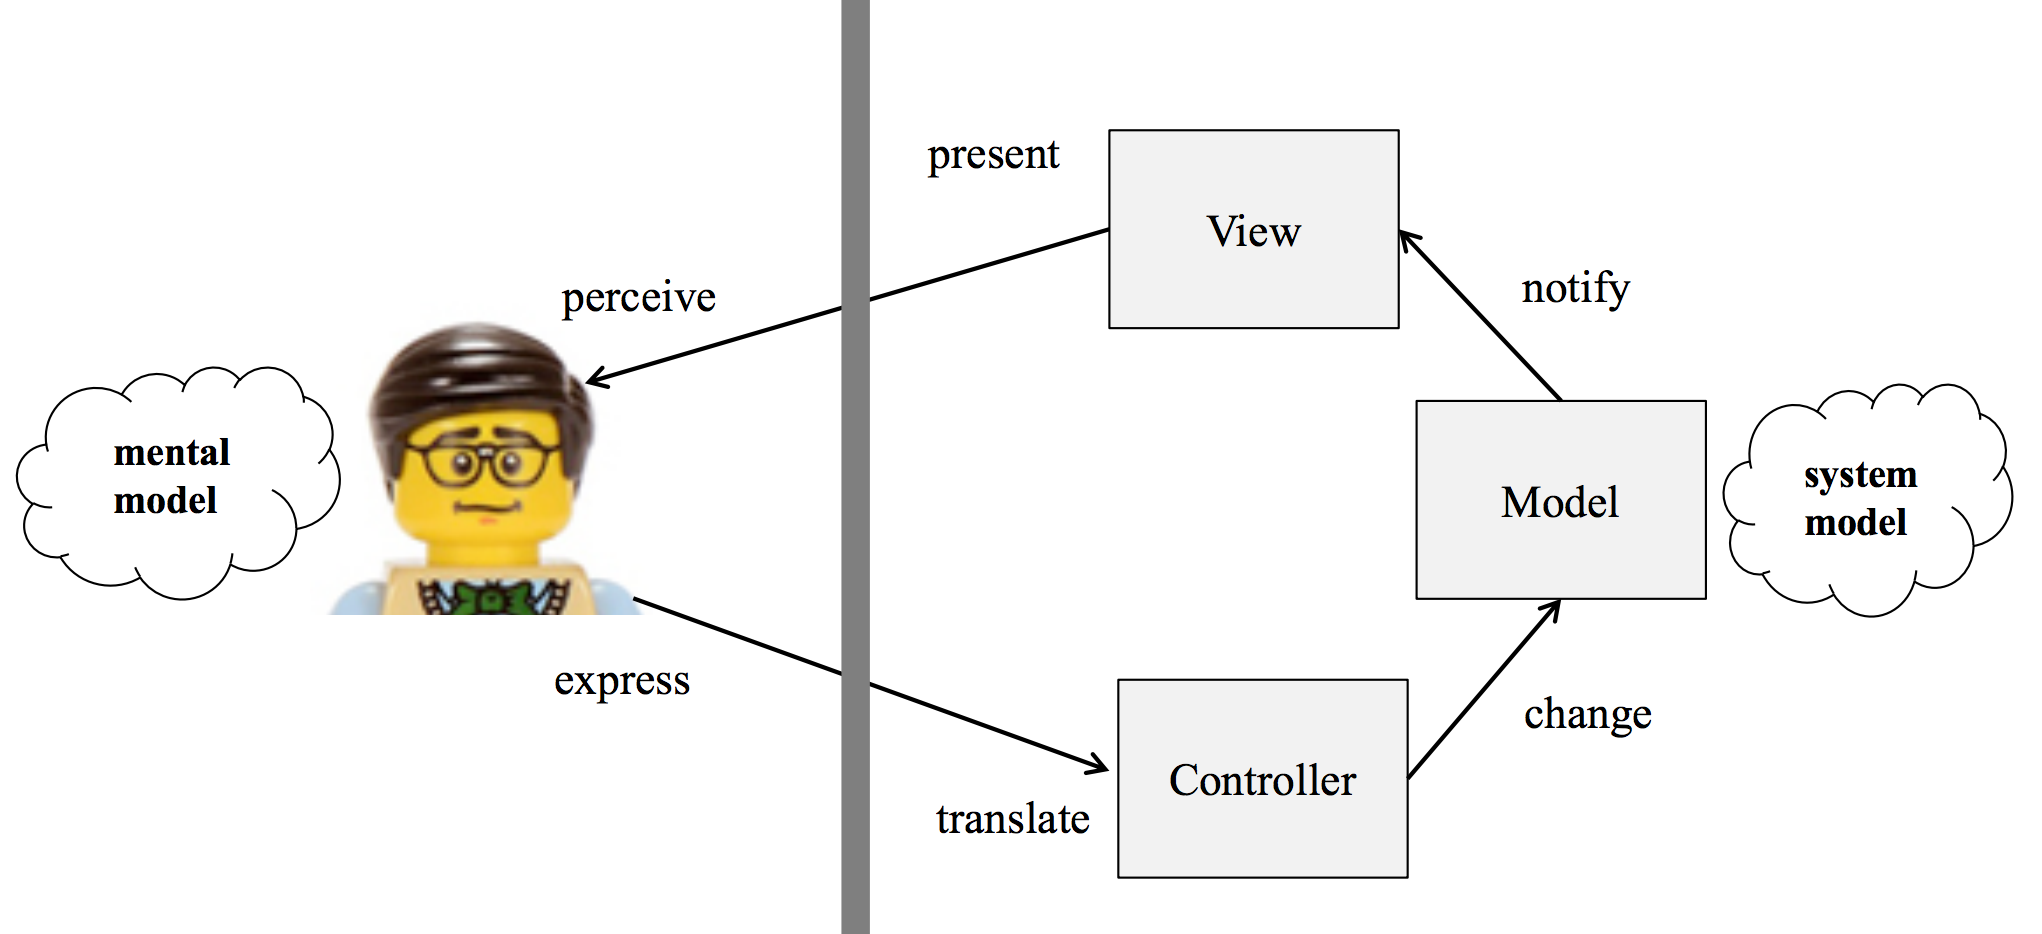
\includegraphics[width=0.7\textwidth]{res/intro_mvc.png}
% \end{figure}

# \textbf{Interface}: external presentation (visual, physical, auditory) to the user
## e.g. controls
# \textbf{Interaction}: actions invoked by user and corresponding responses (behaviour)
## e.g. action and dialog

# Batch interfaces (1945-1965)
## Sets of instructions fed via punch cards
## Only used by highly trained individuals

# Conversationalist interface (1965-1985+)
## Text-based feedback and input
## I/O is in system language, not task language

## Vannevar Bush -- conceptualized the memex, a desk with integrated display, input, and data storage
## Ivan Sutherland -- created the Sketchpad, an early graphical interface with a light pen and direct manipulation
## Douglas Engelbart -- invented the mouse, introduced copy/paste
## Alan Kay -- worked on the Xerox Star, first commercial computer with GUI

# Graphic user interface (1984+)
## Hardware interface: high resolution \& refresh graphics display, keyboard, and pointing device
## WIMP interface: windows, icons, menus, and pointer
## Benefits of GUI:
### Keeps the user in control
### Emphasize recognition (discovery of options) over recall (memorizing commands)
### Uses metaphor; makes interaction language closer to user's language

\end{easylist}

\newpage
\subsection*{Windowing Systems \& X11}
\begineasylist

# \textbf{Windowing system}: provides input, output, and window management capabilities to the OS

# \textbf{X Windows (X11)}:
## Standard windowing system for Unix-based systems

# X11 architecture
## \textbf{X Client} handles all application logic
## \textbf{X Server} handles all user input \& display output
## There may be many clients -- each client is an application; server draws all clients onto one screen and reads all input \\
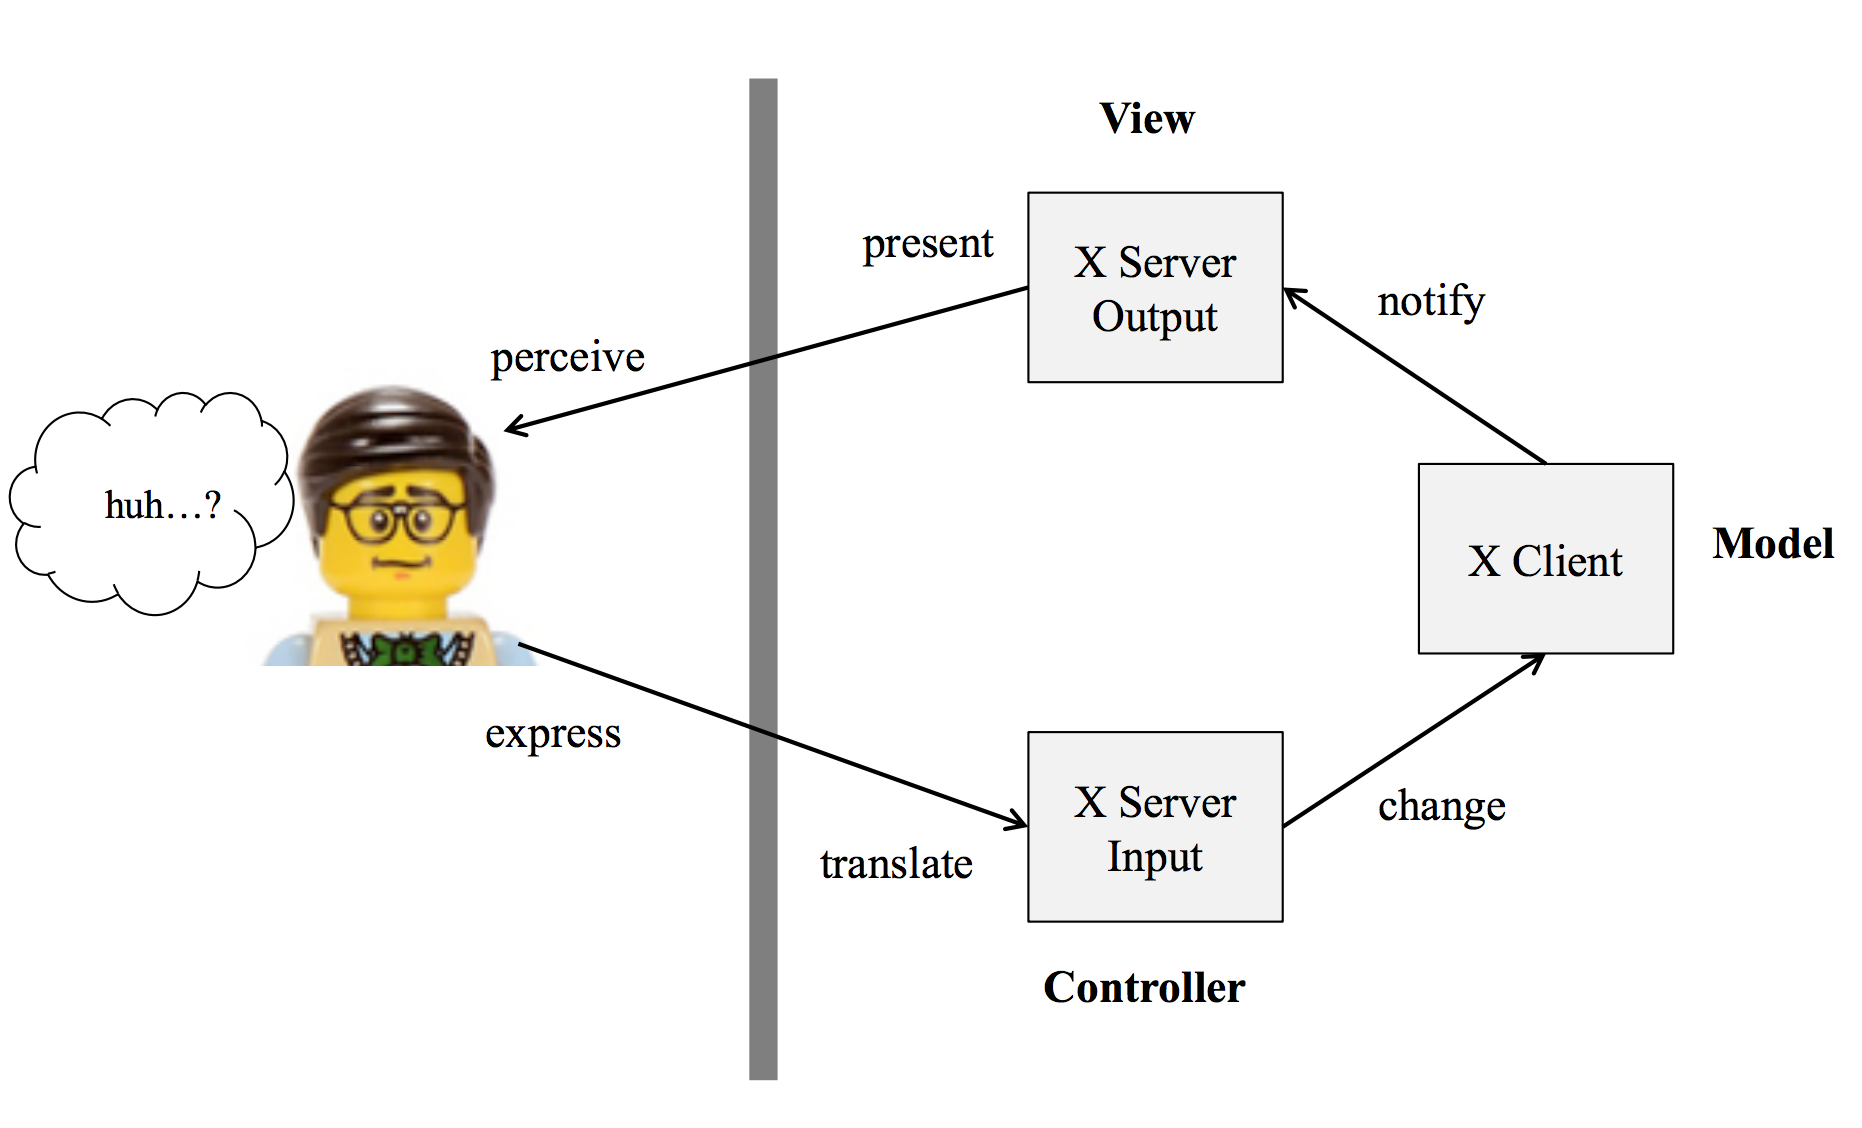
\includegraphics[width=0.7\textwidth]{res/mvc_x11.png}

# Structure of an X program (application is run on the X client):
## Perform client initialization
## Connect to X server (e.g. \texttt{XOpenDisplay()}, \texttt{XCreateWindow()})
## Perform X related initialization (e.g. create graphic contexts with \texttt{XCreateGC()}; put window on the screen with \texttt{XMapRaised()})
## Event loop
### Get next event from server (e.g. \texttt{XNextEvent()})
### Handle event (e.g. \texttt{XLookupKeysym()})
### Send draw request to server (e.g. flush output buffer with \texttt{XFlush()})
## Close down connection to X server (e.g. \texttt{XCloseDisplay()})
## Perform client cleanup

# X11 is a \textbf{base windowing system}: \\
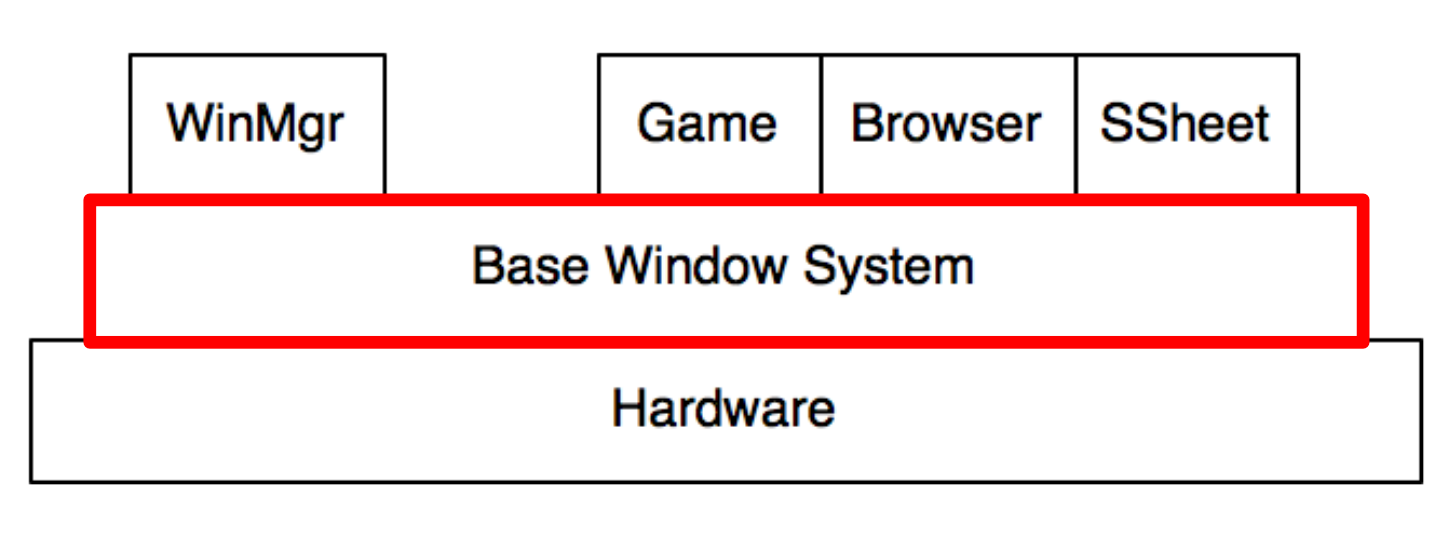
\includegraphics[width=0.5\textwidth]{res/bws.png}
## A standard/protocol for creating windows, low-level graphical output, and user input
## Does not specify the style of each application's UI
## Provides each application with a window and manages its access
## Each application (only) owns a \un{canvas}; shielded from details such as visibility, other windows, etc.

## Some \un{design goals} of X11/BWS:
### Supports multiple overlapping \& resizable windows
### A display may have multiple screens (e.g. monitors) and a window may span multiple screens
### High-performance, high-quality text, 2D graphic \& imaging

# \textbf{Window manager}:
## Provides interactive components (e.g. menus, close button, resizing)
## The WM owns each application's window itself (while application owns the canvas)
### i.e. application developers usually cannot change the window style
## Separation of the WM from the BWS enables many alternative ``look and feels'' \\
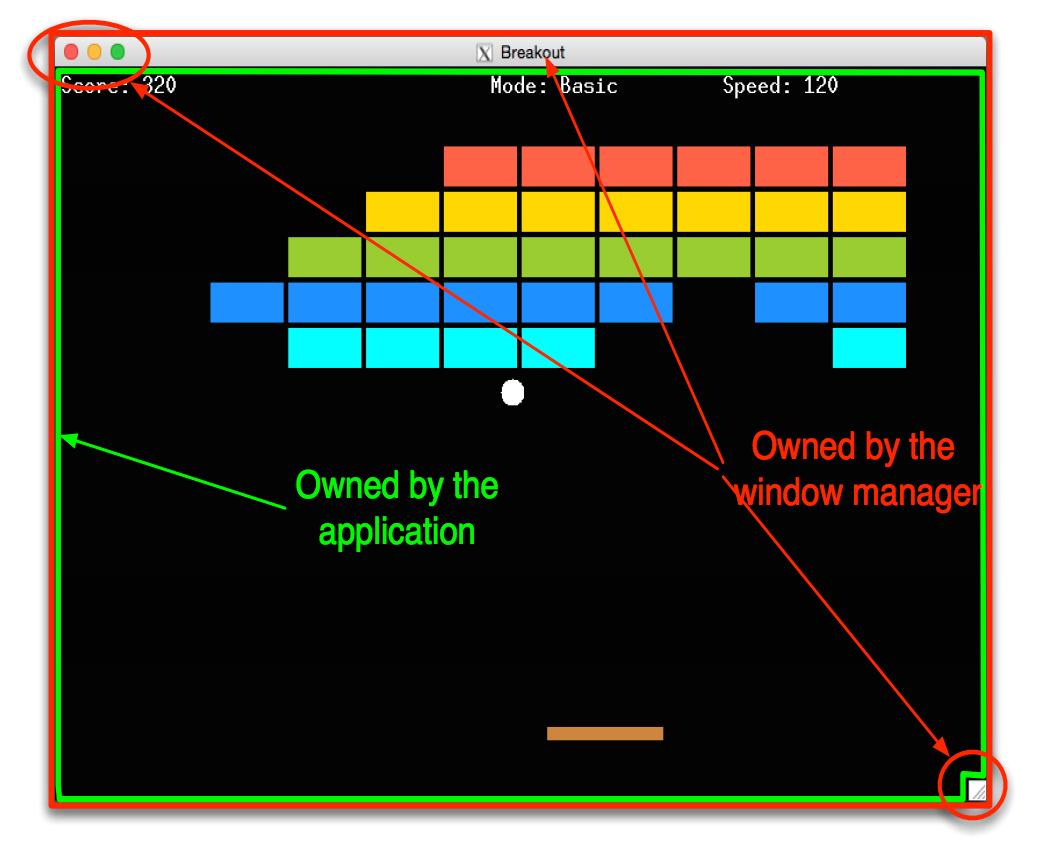
\includegraphics[width=0.5\textwidth]{res/wm.png}

# \textbf{Drawing}
## Three conceptual drawing models:
### Pixel (e.g. images)
### Stroke (e.g. lines, outlines of shapes)
### Region (e.g. text, filled shapes)

## X11 uses \un{graphics contexts} to store drawing options/parameters -- stored on X server

## \textbf{Clipping}: exposing only a particular region (specified by a mask) of an underlying image
## Implementation in X11:
### \texttt{XSetClipMask()}, \texttt{XSetClipRectangles()}
### Only exposed area is repainted

## \textbf{Painter's Algorithm}: draw shapes in layers from back to front to create composite shapes
## Implementation in X11:
### \texttt{Displayable} class with abstract \texttt{paint()} method
### Implement \texttt{paint()} in each subclass
### Draw list of \texttt{Displayables} from back to front, clear screen on every repaint

# \textbf{Events \& animation}
## Objective: need to map input from real-word devices to actions within a system
## \un{Event-driven programming}: flow of program is determined by \un{events} such as user input (key press, mouse click, input focus change) or sensor/timer events
## Implementation in X11:
### Use \texttt{XSelectInput()} and event masks (e.g. \texttt{KeyPressMask} etc.) to register for types of events 
### Use \texttt{XNextEvent()} to dequeue the next event; \un{may block if no events}
#### Use \texttt{XPending()} to check for \# of events before dequeueing
### Should dequeue \emph{all events} before repainting to avoid input lag
### Should subtract time spent in event loop from \texttt{sleep()} to maintain consistent FPS
### Should draw all images to a \emph{buffer} (\texttt{XCreatePixmap()}), then copy the buffer onto the screen in one go (\texttt{XCopyArea()}) (aka. \un{double buffering})
#### Avoids displaying an intermediate image (i.e. flickering)

\end{easylist}

\newpage
\subsection*{Widgets, Events \& Layout}
\begineasylist

# \textbf{Widgets}: parts of an interface that have their own behaviour
## Control their own appearance; recieve and handle their own events
## Widgets \un{toolkit} defines a set of GUI components
## Design goals: 
### \emph{Complete} -- covers wide range of functionality
### \emph{Consistent} -- look-and-feel across components
### \emph{Customizable} -- developers can extend functionality

## Consistent behaviour of components helps users anticipate how the interface will react, and promotes easier \emph{discoverability} of features

\hspace{-2em}
\begin{tabular}{|l|l|}
\hline
\begin{minipage}[t]{0.45\textwidth}
Heavyweight widgets:
    \begin{itemized}
    \item Wrappers around OS's native GUI \& windowing system 
    \item e.g. Java AWT
    \end{itemized}
    \vspace*{0.5em}
\end{minipage}
&
\begin{minipage}[t]{0.45\textwidth}
Lightweight widgets:
    \begin{itemized}
    \item OS provides top-level window in which widgets are drawn
    \item Toolkit is responsible to passing events to widgets
    \end{itemized}
    \vspace*{0.5em}
\end{minipage}  \\
\hline
\begin{minipage}[t]{0.45\textwidth}
Advantages:
    \begin{itemized}
    \item Events passed directly to OS/BWS
    \item Preserves the OS look-and-feel
    \end{itemized}
    \vspace*{0.5em}
\end{minipage}
&
\begin{minipage}[t]{0.45\textwidth}
Advantages:
    \begin{itemized}
    \item Consistent look-and-feel across platforms
    \item Consistent widget set across platforms
    \item Allows for highly optimized widgets
    \end{itemized}
    \vspace*{0.5em}
\end{minipage}  \\
\hline
\begin{minipage}[t]{0.45\textwidth}
Disadvantages:
    \begin{itemized}
    \item OS-specific programming
    \item Small set of common widgets across different platforms
    \end{itemized}
    \vspace*{0.5em}
\end{minipage}
&
\begin{minipage}[t]{0.45\textwidth}
Disadvantages:
    \begin{itemized}
        \item May appear ``non-native''
    \end{itemized}
    \vspace*{0.5em}
\end{minipage}  \\
\hline
\end{tabular} \\

# Widgets as logical input devices
## Characteristics:
### \un{Model} manipulated by the widget (e.g. number, text)
### \un{Events} generated by the widget (e.g. changed)
### \un{Properties} (behaviour and appearance) of the widget (e.g. colour, size, allowed values) \\
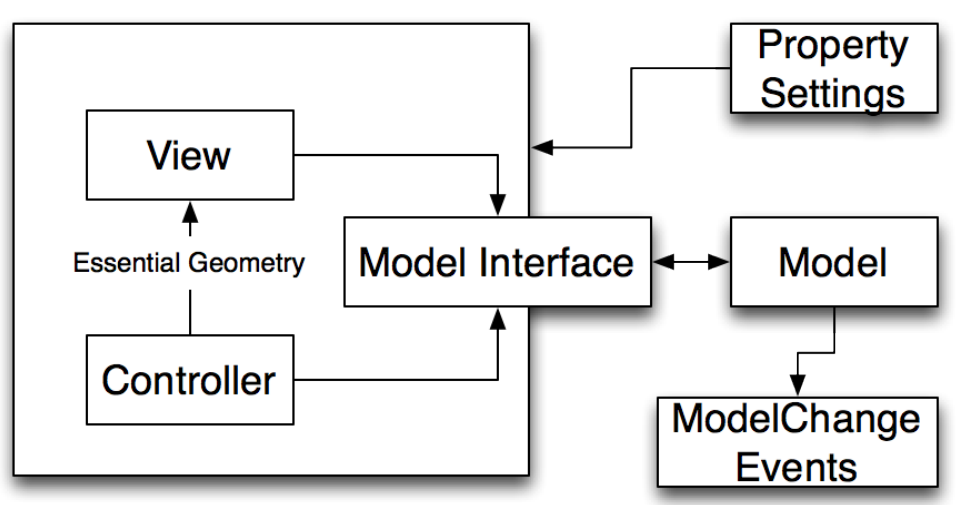
\includegraphics[width=0.5\textwidth]{res/mvc_widget.png}

## Model is abstracted into an interface/abstract class for more code reuse and customizability
### Interface may provide many accessors, mutators \& event-firing functions to be implemented by the custom widgets, allowing for easy manipulation of custom data

## Examples of widgets and their characterstics:
### e.g. button
#### Model = \emph{none}; events = \emph{push}; properties = \emph{label, size, colour etc.}
### e.g. radio button
#### Model = \emph{Boolean}; events = \emph{changed}; properties = \emph{size, colour etc.}
### e.g. text field
#### Model = \emph{string}; events = \emph{changed, selection}; properties = \emph{optional formatters, font etc.}
## Special value widgets: colour picker, calendar etc.


# Event dispatch $\rightarrow$ event handling $\rightarrow$ notifying view \& windowing system

# \textbf{Event dispatch}: dequeueing events from event queue and pushing to appropriate applications

## \un{Interactor tree} -- hierarchy of containers and their nested widgets

## \un{Positional dispatch} -- input sent to widget under mouse cursor location
### Bottom-up positional dispatch:
#### Event routed to leaf widget in interactor tree
#### Widget can process the event or pass to its parent
#### e.g. widget belongs in a group/container -- may be better for container to handle the event
### Top-down positional dispatch:
#### Event routed to highest-level node that contains mouse cursor
#### Widget can process the event or pass to child component
#### e.g. parent widget can enforce policies
#### e.g. easy logging of events (as it traverses down through the tree)

## \un{Focus dispatch} -- events dispatched to widget that has keyboard/mouse focus
### At most one widget each can be in keyboard \& mouse focus at a given time
## Focus dispatch also needs positional dispatch to change focus
## Accelerator keys can bypass focus dispatch

\hspace{-2em}
\begin{tabular}{|l|l|}
\hline
\begin{minipage}[t]{0.45\textwidth}
Heavyweight toolkits:
    \begin{itemized}
    \item BWS has visibility to all widgets
    \item Can use top-down or bottom-up dispatch
    \end{itemized}
    \vspace*{0.5em}
\end{minipage}
&
\begin{minipage}[t]{0.45\textwidth}
Lightweight toolkits:
    \begin{itemized}
    \item BWS only has visibility to application window
    \item Toolkit dispatches event to widget
    \item Can only use top-down dispatch
    \end{itemized}
    \vspace*{0.5em}
\end{minipage}  \\
\hline
\end{tabular} \\

# \textbf{Event handling}: interpreting events in widget's application code
## Event loop \& switch statement (X11):
### All events are consumed in one event loop
### Switch statement selects the appropriate code for each event (\texttt{switch (event.type) \ldots})
### Downsides: switch statement needs to encompass every type of event (too many!)

## Inheritance binding (Java, OS X):
### Events are dispatched to base widget class with predefined event handling methods (default behaviour)
### Child widget overrides methods with custom behaviour
### Downsides:
#### Multiple events are handled by each method -- becomes switch statement again
#### Event handling code in application logic (child widget) -- no separation of concerns
#### Difficult to add new events

## Listener binding (Java):
### \un{Interface binding} -- widget class implements event listener interfaces

\hspace{2em} \texttt{public class A implements Listener \{ // implement all methods \}}

### \un{Object binding} -- widget class holds listener objects (implement listener interface as a nested class)
#### Event handling \& application code are decoupled

\texttt{this.addListener(new Listener() \{ // implement all methods \});}

### \un{Adapter pattern} -- widget class holds adapter objects (class with boilerplate implementations)
#### Custom adapter only needs to extend methods that are used

\texttt{this.addListener(new ListenerAdapter() \{ // override some methods \});}

## Delegate binding (.NET):
### Delegates ``point'' to a method (or methods); invoking delegate calls all associates methods

\hspace{2em} \texttt{delegate = object.Method1; delegate += object.Method2; delegate(args);} \\


# \textbf{Layouts}:
## Dynamic layout: 

\end{easylist}

\newpage
\subsection*{Graphics \& Transformations}
\begineasylist

#






\end{easylist}

\end{document}
